\subsection{Spot Lights}

\begin{frame}{Spot Lights - Introduction}
  \begin{columns}
    \begin{column}{0.7\textwidth}
      \begin{raybox}{Spot Light Characteristics}
        Light emanating from a point within a cone

        \only<2>{
          \vspace{0.1cm}
          \textbf{Real-world examples:}
          \begin{itemize}
            \item Flashlights, headlights
            \item Stage spotlights
            \item Desk lamps
          \end{itemize}
        }
      \end{raybox}

      \only<3>{
        \begin{center}
          \begin{figure}
            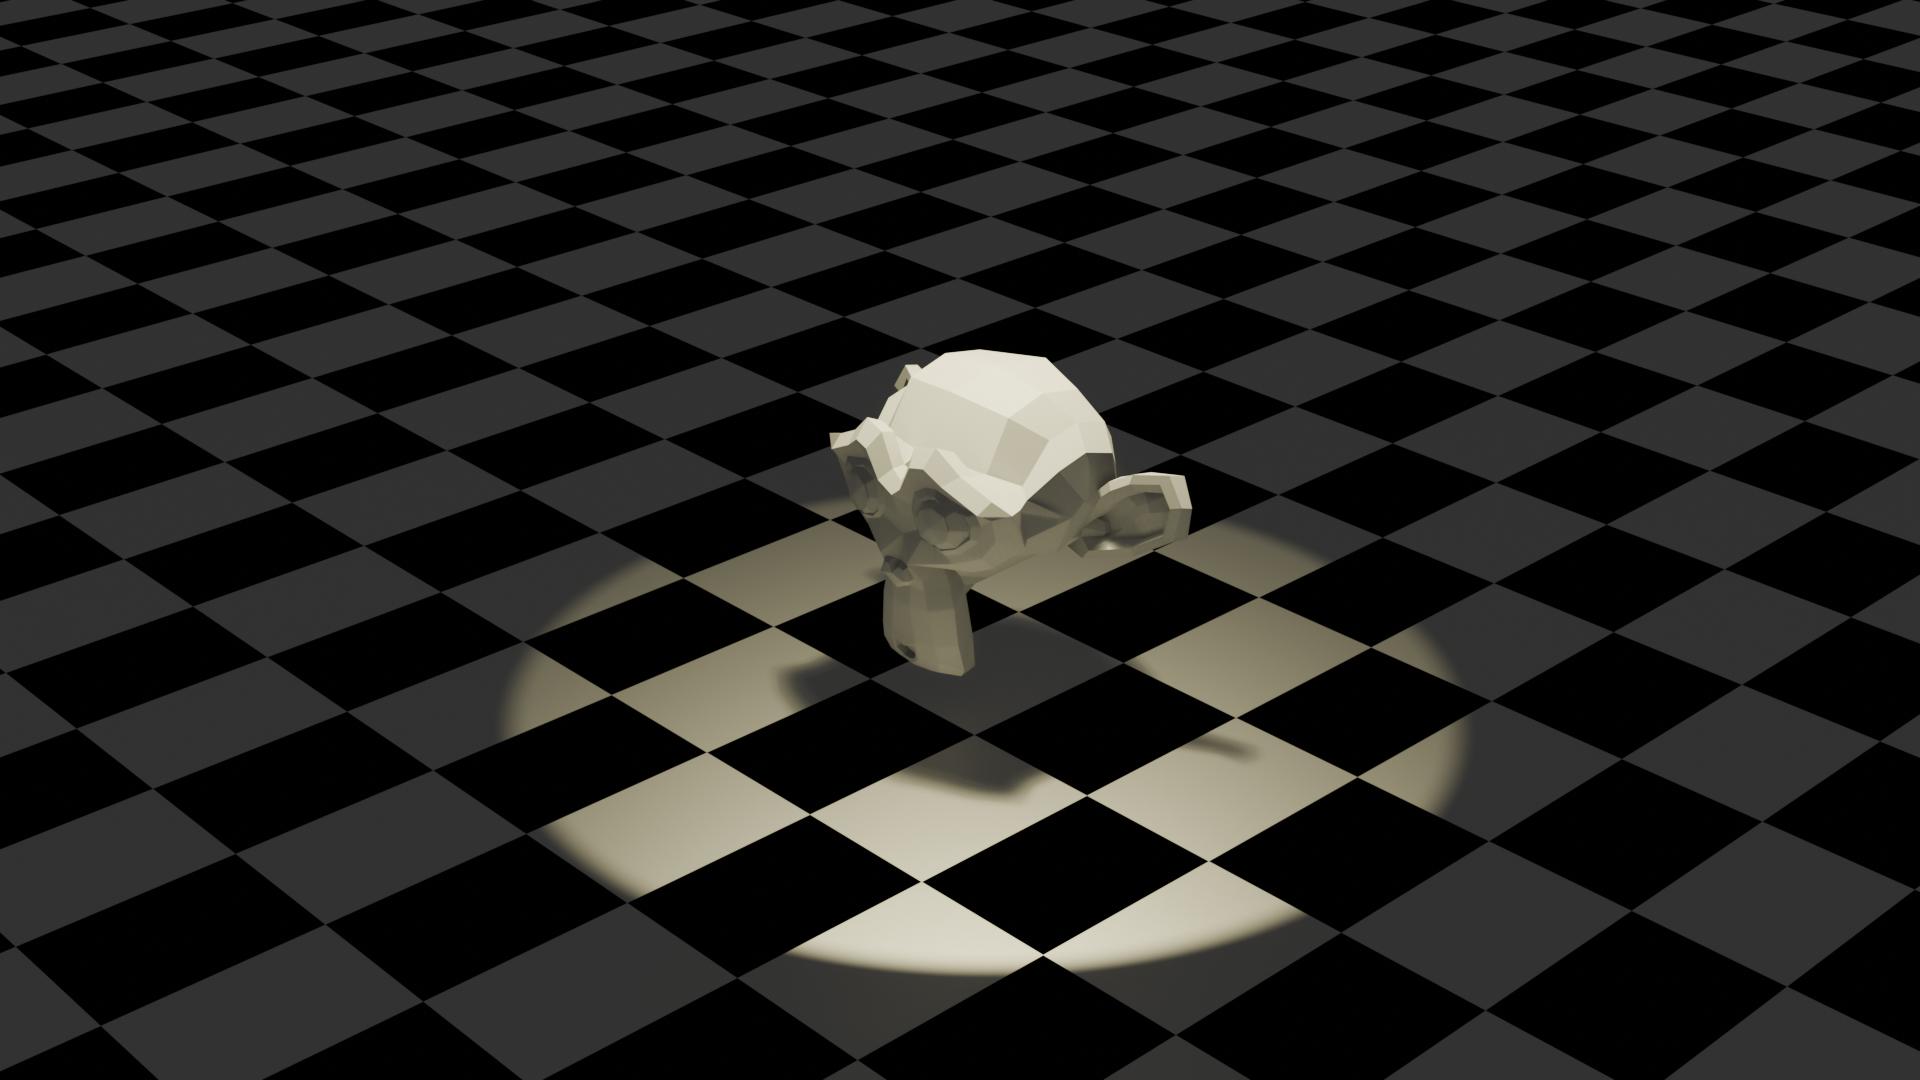
\includegraphics[width=\linewidth]{images/spot.png}
            \caption*{Spot Light ft. Suzanne the monkey}
          \end{figure}
        \end{center}
      }
    \end{column}
    \begin{column}{0.3\textwidth}
      \centering
      \begin{tikzpicture}[scale=0.8]
        \node[circle, fill=LightColor, minimum size=0.6cm] (light) at (1,3) {\footnotesize S};
        \node[above] at (1,3.5) {\footnotesize Spotlight};

        \draw[lightray, thick] (light) -- (0,0);
        \draw[lightray, thick] (light) -- (2,0);
        \draw[lightray, fill=LightColor, opacity=0.2] (light.center) -- (0,0) -- (2,0) -- cycle;

        \draw[->, red, very thick] (light) -- (1,1.5);
        \node[right] at (1.2,2.2) {\footnotesize Direction};

        \draw[-] (1, 1.25) arc [start angle=-90, end angle=-71, radius=1.75] node[midway, below] {\footnotesize $\theta$};

        \draw[dashed] (light) -- (1,0);

        \node[sphere, minimum size=0.6cm] (obj1) at (0.7,-0.5) {};
        \node[sphere, minimum size=0.6cm,fill=ObjectColor!60] (obj2) at (3,-0.5) {};

        \node[below] at (0.7,-1) {\footnotesize Lit};
        \node[below] at (3,-1) {\footnotesize Dark};
      \end{tikzpicture}
    \end{column}
  \end{columns}
\end{frame}

\begin{frame}{Spot Light Mathematics - Cone Calculation}
  \begin{columns}
    \begin{column}{0.7\textwidth}
      \begin{mathbox}{Spot Light Parameters}
        \textbf{Position:} $\mathbf{P}_l$

        \textbf{Intensity:} $\mathbf{I}_l$

        \textbf{Direction:} $\mathbf{D}_{\text{spot}}$

        \textbf{Cone angle:} $\theta_{\text{cutoff}}$

        \textbf{Falloff exponent:} $e$

        \vspace{0.3cm}
        \pause
        \textbf{Step 1 - Calculate angle to surface:}
        \begin{align*}
          \hat{\mathbf{L}} &= \frac{\mathbf{P}_l - \mathbf{P}_{\text{surface}}}
          {|\mathbf{P}_l - \mathbf{P}_{\text{surface}}|} \\
          \cos(\alpha) &=  \mathbf{D}_{\text{spot}} \cdot (- \hat{\mathbf{L}})
        \end{align*}

        \pause
        \textbf{Step 2 - Check if inside cone:}
        \begin{align*}
          \text{if } \cos(\alpha) > \cos(\theta_{\text{cutoff}}) \text{ then illuminate}
        \end{align*}
      \end{mathbox}
    \end{column}
    \begin{column}{0.3\textwidth}
      \begin{tikzpicture}[scale=0.8]
        \node[circle, fill=LightColor, minimum size=0.6cm] (light) at (3,3) {\footnotesize S};

        \begin{scope}[plane origin={(1,1,0)},
            plane x={(0.293,1.707,0)},
            plane y={(1,1,1)},
          canvas is plane]
          \draw[ObjectColor, fill=ObjectColor!20, opacity=0.6] (0,0) circle (1);
        \end{scope}

        \coordinate (surface) at (1,1);
        \fill[ObjectColor] (1,1) circle (2pt);
        \node[below] at (1,1) {\footnotesize $\mathbf{P}_{\text{surface}}$};

        \begin{scope}[shift={(3,3)}]

          \draw[->, blue, thick] (light) -- ($(light)+0.5*(surface)-0.5*(light)$) node[midway, above, anchor=south, black, xshift=-0.1cm] {\footnotesize $-\hat{\mathbf{L}}$};

          \draw[dashed] (light) -- (surface);
          \draw[dashed] (light) -- (-90:5);

          \draw[-] (0,-1) arc [start angle=-90, end angle=-135, radius=1] node[midway, below] {\footnotesize $\alpha$};
          \draw[-] (0,-2.5) arc [start angle=-90, end angle=-110, radius=2.5] node[midway, below] {\footnotesize $\theta_{\text{cutoff}}$};

          \draw[lightray, dashed] (light) -- (-70:4);
          \draw[lightray, dashed] (light) -- (-110:4);

          \draw[->, red, very thick] (light) -- (0,-2) node[midway, right, anchor=west, black] {\footnotesize $\mathbf{D}_{\text{spot}}$};
        \end{scope}

      \end{tikzpicture}
    \end{column}
  \end{columns}
\end{frame}

\begin{frame}{Spot Light Attenuation}
  \begin{mathbox}{Complete Spot Light Formula}
    \small
    \textbf{Angular attenuation:}
    \begin{align*}
      \text{spot\_factor} =
      \begin{cases}
        (\cos(\alpha))^e & \text{if } \cos(\alpha) > \cos(\theta_{\text{cutoff}}) \\
        0 & \text{otherwise}
      \end{cases}
    \end{align*}
    \only<2>{
      The $e$ exponent controls how much brighter the light is at the center of the cone compared to the edges.
    }

    \only<3->{
      \textbf{Distance attenuation} (same as point light):
      \begin{align*}
        \text{distance\_attenuation} = \frac{1}{\epsilon + d^2}
      \end{align*}
    }

    \only<4->{
      \textbf{Final intensity:}
      \begin{align*}
        I_{\text{final}} =
        \begin{cases}
          \mathbf{I}_l \cdot (\cos(\alpha))^e \cdot \frac{1}{\epsilon + d^2} & \text{if } \cos(\alpha) > \cos(\theta_{\text{cutoff}}) \\
          0 & \text{otherwise}
        \end{cases}
      \end{align*}
    }
  \end{mathbox}
  \only<2>{
    \begin{figure}
      \centering
      \begin{columns}
        \begin{column}{0.25\textwidth}
          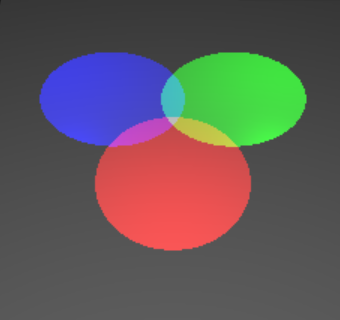
\includegraphics[width=\linewidth]{images/spot_e_0.png}
          \centering
          {\footnotesize $e=0$}
        \end{column}
        \begin{column}{0.25\textwidth}
          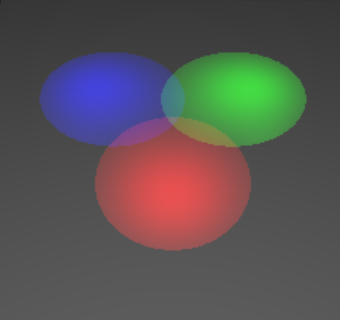
\includegraphics[width=\linewidth]{images/spot_e_10.png}
          \centering
          {\footnotesize $e=10$}
        \end{column}
        \begin{column}{0.25\textwidth}
          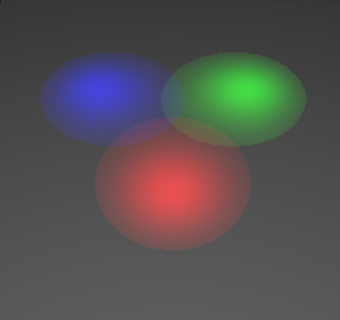
\includegraphics[width=\linewidth]{images/spot_e_20.png}
          \centering
          {\footnotesize $e=20$}
        \end{column}
        \begin{column}{0.25\textwidth}
          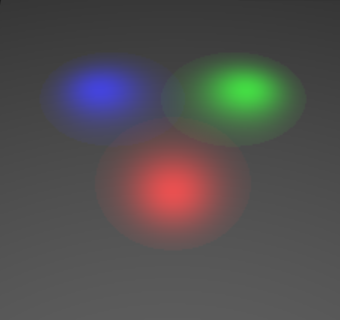
\includegraphics[width=\linewidth]{images/spot_e_30.png}
          \centering
          {\footnotesize $e=30$}
        \end{column}
      \end{columns}
      \caption*{Spot lights for different values of $e$}
    \end{figure}
  }
\end{frame}
